\begin{frame}[fragile]{DT overall structure: simplified example}
  \begin{columns}
    \column{0.6\textwidth}
    \begin{onlyenv}<1>
      \begin{block}{}
\begin{minted}[fontsize=\tiny]{perl}
/ {
  #address-cells = <1>;
  #size-cells = <1>;
  model = "NXP i.MX93 11X11 FRDM board";
  compatible = "fsl,imx93-11x11-frdm", "fsl,imx93";

  cpus { ... };
  reserved-memory { ... };
  chosen { ... };
  gic: interrupt-controller@48000000 { ... };
  soc {
    lpi2c1: i2c@44340000 { ... };
    eqos: ethernet@428a0000 { ... };
  };
};
\end{minted}
      \end{block}
    \end{onlyenv}
    \begin{onlyenv}<2>
      \begin{block}{}
\begin{minted}[fontsize=\tiny]{perl}
/ {
  cpus {
    #address-cells = <1>;
    #size-cells = <0>;

    A55_0: cpu@0 {
      device_type = "cpu";
      compatible = "arm,cortex-a55";
      reg = <0x0>;
      enable-method = "psci";
      #cooling-cells = <2>;
    };

    A55_1: cpu@100 {
      device_type = "cpu";
      compatible = "arm,cortex-a55";
      reg = <0x100>;
      enable-method = "psci";
      #cooling-cells = <2>;
    };
  };

  reserved-memory { ... };
  chosen { ... };
  intc: interrupt-controller@a0021000 { ... };
  soc {
    i2c1: i2c@40012000 { ... };
    ethernet0: ethernet@5800a000 { ... };
  };
};
\end{minted}
      \end{block}
    \end{onlyenv}
    \begin{onlyenv}<3>
      \begin{block}{}
\begin{minted}[fontsize=\tiny]{perl}
/ {
  cpus { ... };
  reserved-memory {
    #address-cells = <2>;
    #size-cells = <2>;
    ranges;

    linux,cma {
      compatible = "shared-dma-pool";
      reusable;
      alloc-ranges = <0 0x80000000 0 0x40000000>;
      size = <0 0x10000000>;
      linux,cma-default;
    };
  };
  chosen {
    bootargs = "console=ttyLP0,115200";
    stdout-path = &lpuart1;
  };
  gic: interrupt-controller@48000000 { ... };
  soc {
    lpi2c1: i2c@44340000 { ... };
    eqos: ethernet@428a0000 { ... };
  };
};
\end{minted}
      \end{block}
    \end{onlyenv}
    \begin{onlyenv}<4>
      \begin{block}{}
\begin{minted}[fontsize=\tiny]{perl}
/ {
  cpus { ... };
  reserved-memory { ... };
  chosen { ... };

  gic: interrupt-controller@48000000 {
      compatible = "arm,gic-v3";
      reg = <0 0x48000000 0 0x10000>,
            <0 0x48040000 0 0xc0000>;
      #interrupt-cells = <3>;
      interrupt-controller;
      interrupts = <GIC_PPI 9 IRQ_TYPE_LEVEL_HIGH>;
      interrupt-parent = <&gic>;
    };

  soc {
    compatible = "simple-bus";
    #address-cells = <1>;
    #size-cells = <1>;
    ranges = <0x0 0x0 0x0 0x80000000>,
       <0x28000000 0x0 0x28000000 0x10000000>;

    lpi2c1: i2c@44340000 { ... };
    eqos: ethernet@428a0000 { ... };
  };
};
\end{minted}
      \end{block}
    \end{onlyenv}
    \begin{onlyenv}<5>
      \begin{block}{}
\begin{minted}[fontsize=\tiny]{perl}
/ {
  cpus { ... };
  reserved-memory { ... };
  chosen { ... };
  gic: interrupt-controller@48000000 { ... };
  soc {
    compatible = "simple-bus";
    ...
    lpi2c1: i2c@44340000 {
      compatible = "fsl,imx93-lpi2c", "fsl,imx7ulp-lpi2c";
      reg = <0x44340000 0x10000>;
      #address-cells = <1>;
      #size-cells = <0>;
      interrupts = <GIC_SPI 13 IRQ_TYPE_LEVEL_HIGH>;
      clocks = <&clk IMX93_CLK_LPI2C1_GATE>,
          <&clk IMX93_CLK_BUS_AON>;
      clock-names = "per", "ipg";
      status = "disabled";
    };
    eqos: ethernet@428a0000 { ... };
  };
};
\end{minted}
      \end{block}
    \end{onlyenv}
    \begin{onlyenv}<6>
      \begin{block}{}
\begin{minted}[fontsize=\tiny]{perl}
/ {
  soc {
    compatible = "simple-bus";
    ...
    lpi2c1: i2c@44340000 { ... };
    eqos: ethernet@428a0000 {
      compatible = "nxp,imx93-dwmac-eqos", "snps,dwmac-5.10a";
      reg = <0x428a0000 0x10000>;
      interrupts = <GIC_SPI 184 IRQ_TYPE_LEVEL_HIGH>,
              <GIC_SPI 183 IRQ_TYPE_LEVEL_HIGH>;
      status = "okay";

      mdio {
        compatible = "snps,dwmac-mdio";
        ...
        ethphy1: ethernet-phy@1 {
          reg = <1>;
          eee-broken-1000t;
          reset-gpios = <&pcal6524 15 GPIO_ACTIVE_LOW>;
          reset-assert-us = <15000>;
          reset-deassert-us = <100000>;
        };
      };
    };
  };
};
\end{minted}
      \end{block}
    \end{onlyenv}
    \column{0.4\textwidth}
    \includegraphics[width=\textwidth]{slides/sysdev-hw-devices/imx93-frdm/simple-hardware-imx93-frdm.pdf}
  \end{columns}
\end{frame}

\begin{frame}[fragile]{Device Tree inheritance}
  \begin{itemize}
  \item Device Tree files are not monolithic, they can be split in
    several files, including each other.
  \item \code{.dtsi} files are included files, while \code{.dts} files
    are {\em final} Device Trees
    \begin{itemize}
    \item Only \code{.dts} files are accepted as input to \code{dtc}
    \end{itemize}
  \item Typically, \code{.dtsi} will contain
    \begin{itemize}
    \item definitions of SoC-level information
    \item definitions common to several boards
    \end{itemize}
  \item The \code{.dts} file contains the board-level information
  \item The inclusion works by {\bf overlaying} the tree of the
    including file over the tree of the included file,
    according to the order of the \code{#include} directives. 
  \item Allows an including file to {\bf override} values specified by
    an included file
  \item Uses the C pre-processor \code{#include} directive
  \end{itemize}
\end{frame}

\begin{frame}{Device Tree inheritance example}
  \begin{center}
    \includegraphics[width=\textwidth]{slides/sysdev-hw-devices/imx93-frdm/dt-inheritance.pdf}
  \end{center}
\end{frame}

\begin{frame}[fragile]{Inheritance and labels}

  \begin{columns}[t]
    \column{0.5\textwidth}
    Doing:
    \begin{block}{soc.dtsi}
      {\tiny
\begin{minted}{perl}
/ {
  soc {
    lpuart1: serial@44380000 {
      compatible = "fsl,imx93-lpuart", "fsl,imx7ulp-lpuart";
      reg = <0x44380000 0x1000>;
      interrupts = <GIC_SPI 19 IRQ_TYPE_LEVEL_HIGH>;
      clocks = <&clk IMX93_CLK_LPUART1_GATE>, ... ;
      clock-names = "ipg", "per";
      status = "disabled";
    };};};
\end{minted}
      }
    \end{block}

    \begin{block}{board.dts}
      {\tiny
\begin{minted}{perl}
#include "soc.dtsi"

/ {
  soc {
    serial@44380000 {
      pinctrl-names = "default";
      pinctrl-0 = <&pinctrl_uart1>;
      status = "okay";
    };};};

\end{minted}
      }
    \end{block}

    \column{0.5\textwidth}
    \begin{onlyenv}<2>
    Is exactly equivalent to:

    \begin{block}{soc.dtsi}
      {\tiny
\begin{minted}{perl}
/ {
  soc {
    lpuart1: serial@44380000 {
      compatible = "fsl,imx93-lpuart", "fsl,imx7ulp-lpuart";
      reg = <0x44380000 0x1000>;
      interrupts = <GIC_SPI 19 IRQ_TYPE_LEVEL_HIGH>;
      clocks = <&clk IMX93_CLK_LPUART1_GATE>, ... ;
      clock-names = "ipg", "per";
      status = "disabled";
    };};};
\end{minted}
      }
    \end{block}

    \begin{block}{board.dts}
      {\tiny
\begin{minted}{perl}
#include "soc.dtsi"

&lpuart1 {
  pinctrl-names = "default";
  pinctrl-0 = <&pinctrl_uart1>;
  status = "okay";
};
\end{minted}
        }
      \end{block}

      $\rightarrow$ this solution is now often preferred
      \end{onlyenv}
  \end{columns}

\end{frame}

\begin{frame}{DT inheritance in imx93-frdm support}
  \begin{center}
    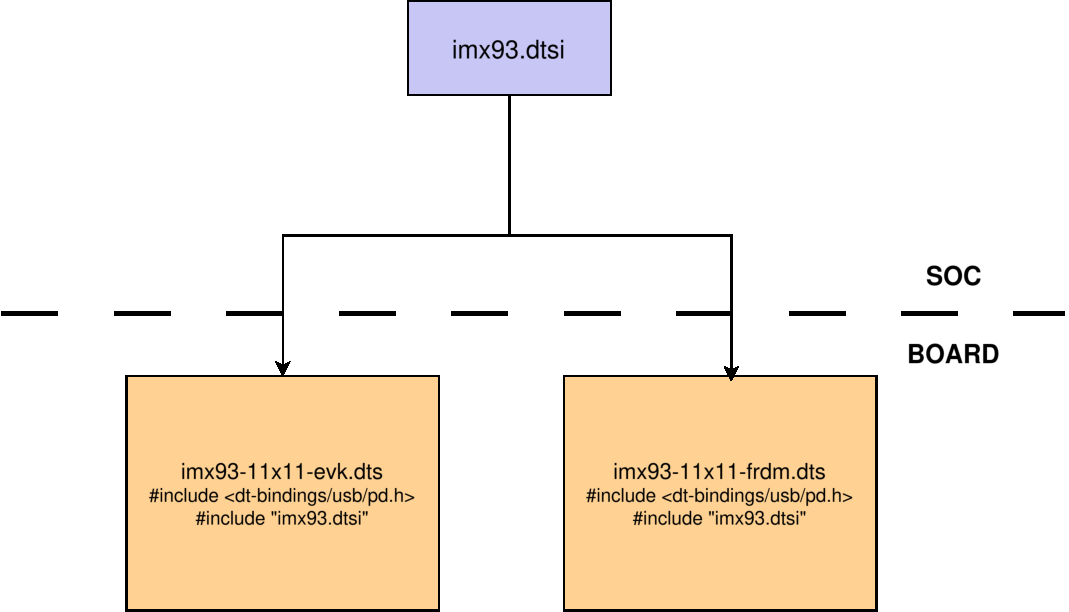
\includegraphics[height=0.8\textheight]{slides/sysdev-hw-devices/imx93-frdm/dt-inheritance-imx93-frdm.pdf}
  \end{center}
\end{frame}

\begin{frame}{DT inheritance in imx6ull-seed-npi-dev-board support}
  \begin{center}
    \includegraphics[height=0.8\textheight]{slides/sysdev-hw-devices/imx93-frdm/dt-inheritance-imx6.pdf}
  \end{center}
\end{frame}

\begin{frame}{Device Tree design principles}
  \begin{itemize}
  \item {\bf Describe hardware} (how the hardware is), not
    configuration (how I choose to use the hardware)
  \item {\bf OS-agnostic}
    \begin{itemize}
    \item For a given piece of HW, Device Tree should be the same for
      U-Boot, FreeBSD or Linux
    \item There should be no need to change the Device Tree when updating the OS
    \end{itemize}
  \item Describe {\bf integration of hardware components}, not the internals
    of hardware components
    \begin{itemize}
    \item The details of how a specific device/IP block is working is
      handled by code in device drivers
    \item The Device Tree describes how the device/IP block is
      connected/integrated with the rest of the system: IRQ lines, DMA
      channels, clocks, reset lines, etc.
    \end{itemize}
  \item Like all beautiful design principles, these principles are
    sometimes violated.
  \end{itemize}
\end{frame}

\begin{frame}{Device Tree specifications}
  \begin{columns}
    \column{0.7\textwidth}
    \begin{itemize}
    \item How to write the correct nodes/properties to describe a
      given hardware platform~?
    \item {\bf Device Tree Specifications} $\rightarrow$ base Device
      Tree syntax + number of standard properties.
      \begin{itemize}
      \item \url{https://www.devicetree.org/specifications/}
      \item Not sufficient to describe the wide variety of hardware.
      \end{itemize}
    \item {\bf Device Tree Bindings} $\rightarrow$ documents that each
      specify how a piece of HW should be described
      \begin{itemize}
      \item \kdir{Documentation/devicetree/bindings} in Linux kernel sources
      \item Reviewed by DT bindings maintainer team
      \item Legacy: human readable documents
      \item New norm: YAML-written specifications
      \end{itemize}
    \end{itemize}
    \column{0.3\textwidth}
    \includegraphics[width=\textwidth]{slides/sysdev-hw-devices/dt-spec.png}
  \end{columns}
\end{frame}

\begin{frame}[fragile]{Device Tree binding: old style}
  \begin{center}
    \kfile{Documentation/devicetree/bindings/mtd/spear_smi.txt}\\
    This IP is {\em not} used on IMX93.
  \end{center}
  \begin{columns}[t]
    \column{0.5\textwidth}
    \begin{block}{}
      {\fontsize{5}{6}\selectfont
\begin{verbatim}
* SPEAr SMI

Required properties:
- compatible : "st,spear600-smi"
- reg : Address range of the mtd chip
- #address-cells, #size-cells : Must be present if the device has sub-nodes
  representing partitions.
- interrupts: Should contain the STMMAC interrupts
- clock-rate : Functional clock rate of SMI in Hz

Optional properties:
- st,smi-fast-mode : Flash supports read in fast mode

\end{verbatim}
      }
    \end{block}
    \column{0.5\textwidth}
    \begin{block}{}
      {\fontsize{4}{5}\selectfont
\begin{verbatim}
Example:

        smi: flash@fc000000 {
                compatible = "st,spear600-smi";
                #address-cells = <1>;
                #size-cells = <1>;
                reg = <0xfc000000 0x1000>;
                interrupt-parent = <&vic1>;
                interrupts = <12>;
                clock-rate = <50000000>;        /* 50MHz */

                flash@f8000000 {
                        st,smi-fast-mode;
                        ...
                };
        };
\end{verbatim}
      }
    \end{block}
  \end{columns}

\end{frame}

\begin{frame}[fragile]{Device Tree binding: YAML style}
  \kfile{Documentation/devicetree/bindings/i2c/i2c-imx-lpi2c.yaml}
  \begin{columns}[t]
    \column{0.5\textwidth}
    \begin{block}{}
      {\fontsize{5}{5}\selectfont
\begin{minted}{yaml}
# SPDX-License-Identifier: (GPL-2.0-only OR BSD-2-Clause)
%YAML 1.2
---
$id: http://devicetree.org/schemas/i2c/i2c-imx-lpi2c.yaml#
$schema: http://devicetree.org/meta-schemas/core.yaml#

title: Freescale Low Power Inter IC (LPI2C) for i.MX

maintainers:
  - Shawn Guo <shawnguo@kernel.org>
  - Sascha Hauer <s.hauer@pengutronix.de>
  - Fabio Estevam <festevam@gmail.com>

allOf:
  - $ref: /schemas/i2c/i2c-controller.yaml#

properties:
  compatible:
    oneOf:
      - enum:
          - fsl,imx7ulp-lpi2c
      - items:
          - enum:
              - fsl,imx8qxp-lpi2c
              - fsl,imx8dxl-lpi2c
              - fsl,imx8qm-lpi2c
              - fsl,imx8ulp-lpi2c
              - fsl,imx93-lpi2c
              - fsl,imx95-lpi2c
          - const: fsl,imx7ulp-lpi2c

  reg:
    maxItems: 1

\end{minted}
      }
    \end{block}
    \column{0.5\textwidth}
    \begin{block}{}
      {\fontsize{5}{5}\selectfont
\begin{minted}{yaml}
  assigned-clock-parents: true
  assigned-clock-rates: true
  assigned-clocks: true
  clock-frequency: true

  clock-names:
    items:
      - const: per
      - const: ipg

  clocks:
    maxItems: 2

  dmas:
    items:
      - description: DMA controller phandle and request line for TX
      - description: DMA controller phandle and request line for RX

  dma-names:
    items:
      - const: tx
      - const: rx

  power-domains:
    maxItems: 1

required:
  - compatible
  - reg
  - interrupts
  - clocks

unevaluatedProperties: false
\end{minted}
      }
    \end{block}
  \end{columns}
\end{frame}

\begin{frame}[fragile]{Device Tree binding: YAML style example}
    \begin{block}{}
      {\fontsize{5}{7}\selectfont
\begin{minted}{yaml}
examples:
  - |
    #include <dt-bindings/clock/imx7ulp-clock.h>
    #include <dt-bindings/interrupt-controller/arm-gic.h>

    i2c@40a50000 {
        compatible = "fsl,imx7ulp-lpi2c";
        reg = <0x40A50000 0x10000>;
        interrupt-parent = <&intc>;
        interrupts = <GIC_SPI 37 IRQ_TYPE_LEVEL_HIGH>;
        clocks = <&clks IMX7ULP_CLK_LPI2C7>,
                 <&clks IMX7ULP_CLK_NIC1_BUS_DIV>;
    };

\end{minted}
      }
    \end{block}
\end{frame}

\begin{frame}{Validating Device Tree in Linux}
  \begin{itemize}
  \item \code{dtc} only does syntactic validation
  \item YAML bindings allow to do semantic validation
  \item Linux kernel \code{make} rules:
    \begin{itemize}
    \item \code{make dt_binding_check}\\
      verify that YAML bindings are valid
    \item \code{make dtbs_check}\\
      validate DTs currently enabled against YAML bindings
    \item \code{make DT_SCHEMA_FILES=Documentation/devicetree/bindings/trivial-devices.yaml dtbs_check}\\
      validate DTs against a specific YAML binding
    \end{itemize}
  \end{itemize}
\end{frame}

\begin{frame}{The {\tt compatible} property}
  \begin{itemize}
  \item Is a list of strings
    \begin{itemize}
    \item From the most specific to the least specific
    \end{itemize}
  \item Describes the specific {\bf binding} to which the node complies.
  \item It uniquely identifies the {\bf programming model} of the
    device.
  \item Practically speaking, it is used by the operating system to
    find the {\bf appropriate driver} for this device.
  \item When describing real hardware, the typical form is
    \code{vendor,model}
  \item Examples:
    \begin{itemize}
    \item \code{compatible = "arm,armv7-timer";}
    \item \code{compatible = "st,stm32mp1-dwmac", "snps,dwmac-4.20a";}
    \item \code{compatible = "regulator-fixed";}
    \item \code{compatible = "gpio-keys";}
    \end{itemize}
  \item Special value: \code{simple-bus} $\rightarrow$ bus where all
    sub-nodes are memory-mapped devices
  \end{itemize}
\end{frame}

\begin{frame}{{\tt compatible} property and Linux kernel drivers}
  \begin{columns}
    \column{0.6\textwidth}
    \begin{itemize}
    \item Linux identifies as {\bf platform devices}:
      \begin{itemize}
      \item Top-level DT nodes with a \code{compatible} string
      \item Sub-nodes of \code{simple-bus}
        \begin{itemize}
        \item Instantiated automatically at boot time
        \end{itemize}
      \end{itemize}
    \item Sub-nodes of I2C controllers $\rightarrow$ {\em I2C devices}
    \item Sub-nodes of SPI controllers $\rightarrow$ {\em SPI devices}
    \item Each Linux driver has a table of compatible strings it supports
      \begin{itemize}
      \item \kstruct{of_device_id}\code{[]}
      \end{itemize}
    \item When a DT node compatible string matches a given driver, the
      device is {\em bound} to that driver.
    \end{itemize}
    \column{0.4\textwidth}
    \includegraphics[width=\textwidth]{slides/sysdev-hw-devices/dt-to-devices.pdf}
  \end{columns}
\end{frame}

\begin{frame}[fragile]{Matching with drivers in Linux: platform driver}
  \begin{block}{\kfile{drivers/tty/serial/fsl_lpuart.c}}
    {\tiny
\begin{minted}{c}
static const struct of_device_id lpuart_dt_ids[] = {
  { .compatible = "fsl,vf610-lpuart",  .data = &vf_data, },
  { .compatible = "fsl,ls1021a-lpuart",  .data = &ls1021a_data, },
  { .compatible = "fsl,ls1028a-lpuart",  .data = &ls1028a_data, },
  { .compatible = "fsl,imx7ulp-lpuart",  .data = &imx7ulp_data, },
  { .compatible = "fsl,imx8ulp-lpuart",  .data = &imx8ulp_data, },
  { .compatible = "fsl,imx8qxp-lpuart",  .data = &imx8qxp_data, },
  { .compatible = "fsl,imxrt1050-lpuart",  .data = &imxrt1050_data},
  { /* sentinel */ }
};
MODULE_DEVICE_TABLE(of, lpuart_dt_ids);

...

static struct platform_driver lpuart_driver = {
  .probe    = lpuart_probe,
  .remove_new  = lpuart_remove,
  .driver    = {
    .name  = "fsl-lpuart",
    .of_match_table = lpuart_dt_ids,
    .pm  = pm_ptr(&lpuart_pm_ops),
  },
};
\end{minted}
    }
  \end{block}
\end{frame}

\begin{frame}[fragile]{Matching with drivers in Linux: I2C driver}
  \begin{block}{\kfile{sound/soc/codecs/cs42l51.c}}
    {\tiny
\begin{minted}{c}
const struct of_device_id cs42l51_of_match[] = {
        { .compatible = "cirrus,cs42l51", },
        { }
};
MODULE_DEVICE_TABLE(of, cs42l51_of_match);
\end{minted}
    }
  \end{block}
  \begin{block}{\kfile{sound/soc/codecs/cs42l51-i2c.c}}
    {\tiny
\begin{minted}{c}
static struct i2c_driver cs42l51_i2c_driver = {
        .driver = {
                .name = "cs42l51",
                .of_match_table = cs42l51_of_match,
                .pm = &cs42l51_pm_ops,
        },
        .probe = cs42l51_i2c_probe,
        .remove = cs42l51_i2c_remove,
        .id_table = cs42l51_i2c_id,
};
\end{minted}
    }
  \end{block}
\end{frame}

\begin{frame}[fragile]{{\tt reg} property}
  \begin{itemize}
  \item Most important property after \code{compatible}
  \item {\bf Memory-mapped} devices: base physical address and size of
    the memory-mapped registers. Can have several entries for multiple
    register areas.
\begin{onlyenv}<1>
\begin{block}{}
\begin{verbatim}
sai4: sai@50027000 {
    reg = <0x50027000 0x4>, <0x500273f0 0x10>;
};
\end{verbatim}
\end{block}
\end{onlyenv}
\pause
  \item {\bf I2C} devices: address of the device on the I2C bus.
\begin{onlyenv}<2>
\begin{block}{}
\begin{verbatim}
&i2c1 {
   hdmi-transmitter@39 {
      reg = <0x39>;
   };
   cs42l51: cs42l51@4a {
      reg = <0x4a>;
   };
};
\end{verbatim}
\end{block}
\end{onlyenv}
\pause
  \item {\bf SPI} devices: chip select number
\begin{onlyenv}<3>
\begin{block}{}
\begin{verbatim}
&qspi {
        flash0: mx66l51235l@0 {
                reg = <0>;
        };
        flash1: mx66l51235l@1 {
                reg = <1>;
        };
};
\end{verbatim}
\end{block}
\end{onlyenv}
\pause
\item The unit address must be the address of the first \code{reg}
  entry.
\begin{onlyenv}<4>
\begin{block}{}
\begin{verbatim}
sai4: sai@50027000 {
    reg = <0x50027000 0x4>, <0x500273f0 0x10>;
};
\end{verbatim}
\end{block}
\end{onlyenv}
  \end{itemize}
\end{frame}

\begin{frame}{Status property}
  \begin{itemize}
  \item The \code{status} property indicates if the device is really in
    use or not
    \begin{itemize}
    \item \code{okay} or \code{ok} $\rightarrow$ the device is really
      in use
    \item any other value, by convention \code{disabled} $\rightarrow$
      the device is not in use
    \end{itemize}
  \item In Linux, controls if a device is instantiated
  \item In \code{.dtsi} files describing SoCs: all devices that
    interface to the outside world have \code{status = "disabled";}
  \item Enabled on a per-device basis in the board \code{.dts}
  \end{itemize}
\end{frame}

\begin{frame}[fragile]{Resources: interrupts, clocks, DMA, reset lines, ...}
  \begin{columns}
  \column{0.5\textwidth}
  \begin{itemize}
  \item Common pattern for resources shared by multiple hardware
    blocks
    \begin{itemize}
    \item Interrupt lines
    \item Clock controllers
    \item DMA controllers
    \item Reset controllers
    \item ...
    \end{itemize}
  \item A Device Tree node describing the {\em controller} as a device
  \item References from other nodes that use resources provided by
    this {\em controller}
  \end{itemize}
  \column{0.5\textwidth}
\begin{block}{}
{\fontsize{4}{5}\selectfont
\begin{minted}{perl}
gic: interrupt-controller@48000000 {
  compatible = "arm,gic-v3";
  reg = <0 0x48000000 0 0x10000>,
        <0 0x48040000 0 0xc0000>;
  #interrupt-cells = <3>;
  interrupt-controller;
  interrupts = <GIC_PPI 9 IRQ_TYPE_LEVEL_HIGH>;
  interrupt-parent = <&gic>;
};

clk: clock-controller@44450000 {
  compatible = "fsl,imx93-ccm";
  reg = <0x44450000 0x10000>;
  #clock-cells = <1>;
  clocks = <&osc_32k>, <&osc_24m>, <&clk_ext1>;
  clock-names = "osc_32k", "osc_24m", "clk_ext1";
};

edma1: dma-controller@44000000 {
  compatible = "fsl,imx93-edma3";
  reg = <0x44000000 0x200000>;
  #dma-cells = <3>;
  dma-channels = <31>;
  interrupts = <GIC_SPI 95 IRQ_TYPE_LEVEL_HIGH>, <GIC_SPI 96 IRQ_TYPE_LEVEL_HIGH>;
  clocks = <&clk IMX93_CLK_EDMA1_GATE>;
  clock-names = "dma";
};

lpuart1: serial@44380000 {
  compatible = "fsl,imx93-lpuart", "fsl,imx8ulp-lpuart", "fsl,imx7ulp-lpuart";
  reg = <0x44380000 0x1000>;
  interrupts = <GIC_SPI 19 IRQ_TYPE_LEVEL_HIGH>;
  clocks = <&clk IMX93_CLK_LPUART1_GATE>;
  clock-names = "ipg";
  dmas = <&edma1 17 0 FSL_EDMA_RX>, <&edma1 16 0 0>;
  dma-names = "rx", "tx";
};
\end{minted}
}
\end{block}
\end{columns}
\end{frame}

\begin{frame}{Pin-muxing description}
  \begin{columns}
    \column{0.5\textwidth}
    \begin{itemize}
    \item Most modern SoCs, including the IMX93, have more features
      than they have pins to expose those features to the outside world.
    \item Pins are muxed: a given pin can be used for one function
      {\bf or} another
    \item A specific IP block in the SoC controls the muxing of pins:
      the {\bf pinmux controller}
    \item The Device Tree describes which pin configurations are
      possible, and which configurations are used by the different
      devices.
    \end{itemize}
    \column{0.5\textwidth}
    \includegraphics[width=\textwidth]{slides/sysdev-hw-devices/pin-muxing-principle.pdf}
  \end{columns}
\end{frame}

\begin{frame}[fragile]{Pin-muxing controllers on IMX93}
  \begin{block}{\kfileversion{arch/arm64/boot/dts/freescale/imx93-11x11-frdm.dts}{6.1}}
{\tiny
\begin{minted}{perl}
iomuxc: pinctrl@443c0000 {
    compatible = "fsl,imx93-iomuxc";
    reg = <0x443c0000 0x10000>;
    pinctrl_uart1: uart1grp {
        fsl,pins = <
            MX93_PAD_UART1_RXD__LPUART1_RX 0x31e
            MX93_PAD_UART1_TXD__LPUART1_TX 0x31e
        >;
    };
    pinctrl_lpi2c1: lpi2c1grp {
        fsl,pins = <
            MX93_PAD_I2C1_SCL__LPI2C1_SCL 0x40000b9e
            MX93_PAD_I2C1_SDA__LPI2C1_SDA 0x40000b9e
        >;
    };
};

lpuart1: serial@44380000 {
    compatible = "fsl,imx93-lpuart", "fsl,imx8ulp-lpuart", "fsl,imx7ulp-lpuart";
    reg = <0x44380000 0x1000>;
    interrupts = <GIC_SPI 19 IRQ_TYPE_LEVEL_HIGH>;
    clocks = <&clk IMX93_CLK_LPUART1_GATE>;
    clock-names = "ipg";
    pinctrl-names = "default";
    pinctrl-0 = <&pinctrl_uart1>;
    status = "okay";
};
\end{minted}
}
  \end{block}
\end{frame}

\begin{frame}[fragile]{Pin-muxing configuration}
\begin{onlyenv}<1>
  \begin{block}{\kfile{arch/arm64/boot/dts/freescale/imx93-11x11-frdm.dts}}
{\tiny
\begin{minted}{perl}
&iomuxc {
    pinctrl_lpi2c1: lpi2c1grp {
        fsl,pins = <
            MX93_PAD_I2C1_SCL__LPI2C1_SCL  0x40000b9e
            MX93_PAD_I2C1_SDA__LPI2C1_SDA  0x40000b9e
        >;
    };

    pinctrl_uart1: uart1grp {
        fsl,pins = <
            MX93_PAD_UART1_RXD__LPUART1_RX 0x31e
            MX93_PAD_UART1_TXD__LPUART1_TX 0x31e
        >;
    };

    pinctrl_fec: fecgrp {
        fsl,pins = <
            MX93_PAD_ENET2_MDC__ENET1_MDC      0x57e
            MX93_PAD_ENET2_MDIO__ENET1_MDIO    0x57e
            MX93_PAD_ENET2_RD0__ENET1_RGMII_RD0 0x57e
            ...
        >;
    };
};
\end{minted}
}
\end{block}
\end{onlyenv}
\end{frame}

\begin{frame}[fragile]{Pin-muxing consumer}
  \begin{block}{}
{\tiny
\begin{minted}{perl}
&i2c1 {
        pinctrl-names = "default", "sleep";
        pinctrl-0 = <&i2c1_pins_a>;
        pinctrl-1 = <&i2c1_sleep_pins_a>;
        ...
};
\end{minted}
}
\end{block}
\begin{itemize}
\item Typically board-specific, in \code{.dts}
\item \code{pinctrl-0}, \code{pinctrl-1}, \code{pinctrl-X} provides
  the pin mux configurations for the different {\bf states}
\item \code{pinctrl-names} gives a name to each state, mandatory even
  if only one state
\item States are mutually exclusive
\item The driver is responsible for switching between states
\item \code{default} state is automatically set up when the device is
  {\em probed}
\end{itemize}
\end{frame}

\begin{frame}[fragile]{Example: LED and I2C device}
  \begin{itemize}
  \item Let's see how to describe an LED and an I2C device connected
    to the DK1 platform.
  \item Create \code{arch/arm64/boot/dts/freescale/imx93-11x11-frdm-custom.dts}
    which includes \code{imx93-11x11-frdm.dts}
    \begin{block}{}
{\tiny
\begin{verbatim}
#include "imx93-11x11-frdm.dts"
\end{verbatim}
}
    \end{block}
  \item Make sure \code{imx93-11x11-frdm.dts} gets compiled to a
    DTB by changing \kfile{arch/arm64/boot/dts/freescale/Makefile}
    \begin{block}{}
      {\tiny
\begin{verbatim}
dtb-$(CONFIG_ARCH_MXC) += imx93-11x11-frdm-custom.dtb
\end{verbatim}
      }
    \end{block}
  \item \code{make dtbs}
    \begin{block}{}
      {\tiny
\begin{verbatim}
  DTC     arch/arm64/boot/dts/freescale/imx93-11x11-frdm-custom.dtb
\end{verbatim}
      }
    \end{block}
  \end{itemize}
\end{frame}

\begin{frame}[fragile]{Example: describe an LED}
  \begin{columns}
    \column{0.5\textwidth}
  \begin{block}{imx93-11x11-frdm-custom.dts}
    {\tiny
\begin{minted}{perl}
#include "imx93-11x11-frdm.dts"

/ {
  leds {
    compatible = "gpio-leds";
    webinar {
      label = "webinar";
      gpios = <&gpio2 21 GPIO_ACTIVE_HIGH>;
    };
  };
};
\end{minted}
      }
  \end{block}
  \begin{block}{shell}
{\tiny
\begin{verbatim}
# echo 255 > /sys/class/leds/webinar/brightness
\end{verbatim}
}
\end{block}
  \column{0.5\textwidth}
  \begin{center}
    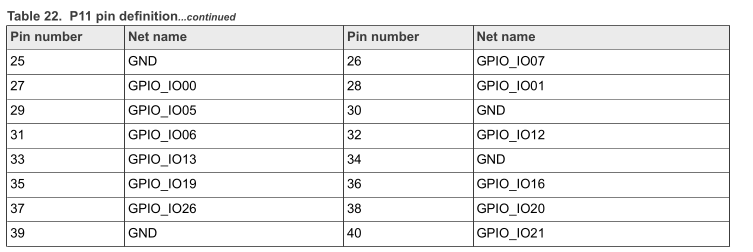
\includegraphics[height=0.3\textheight]{slides/sysdev-hw-devices/imx93-frdm/imx93-tab-gpio21.png}\\
    \vspace{0.5cm}
    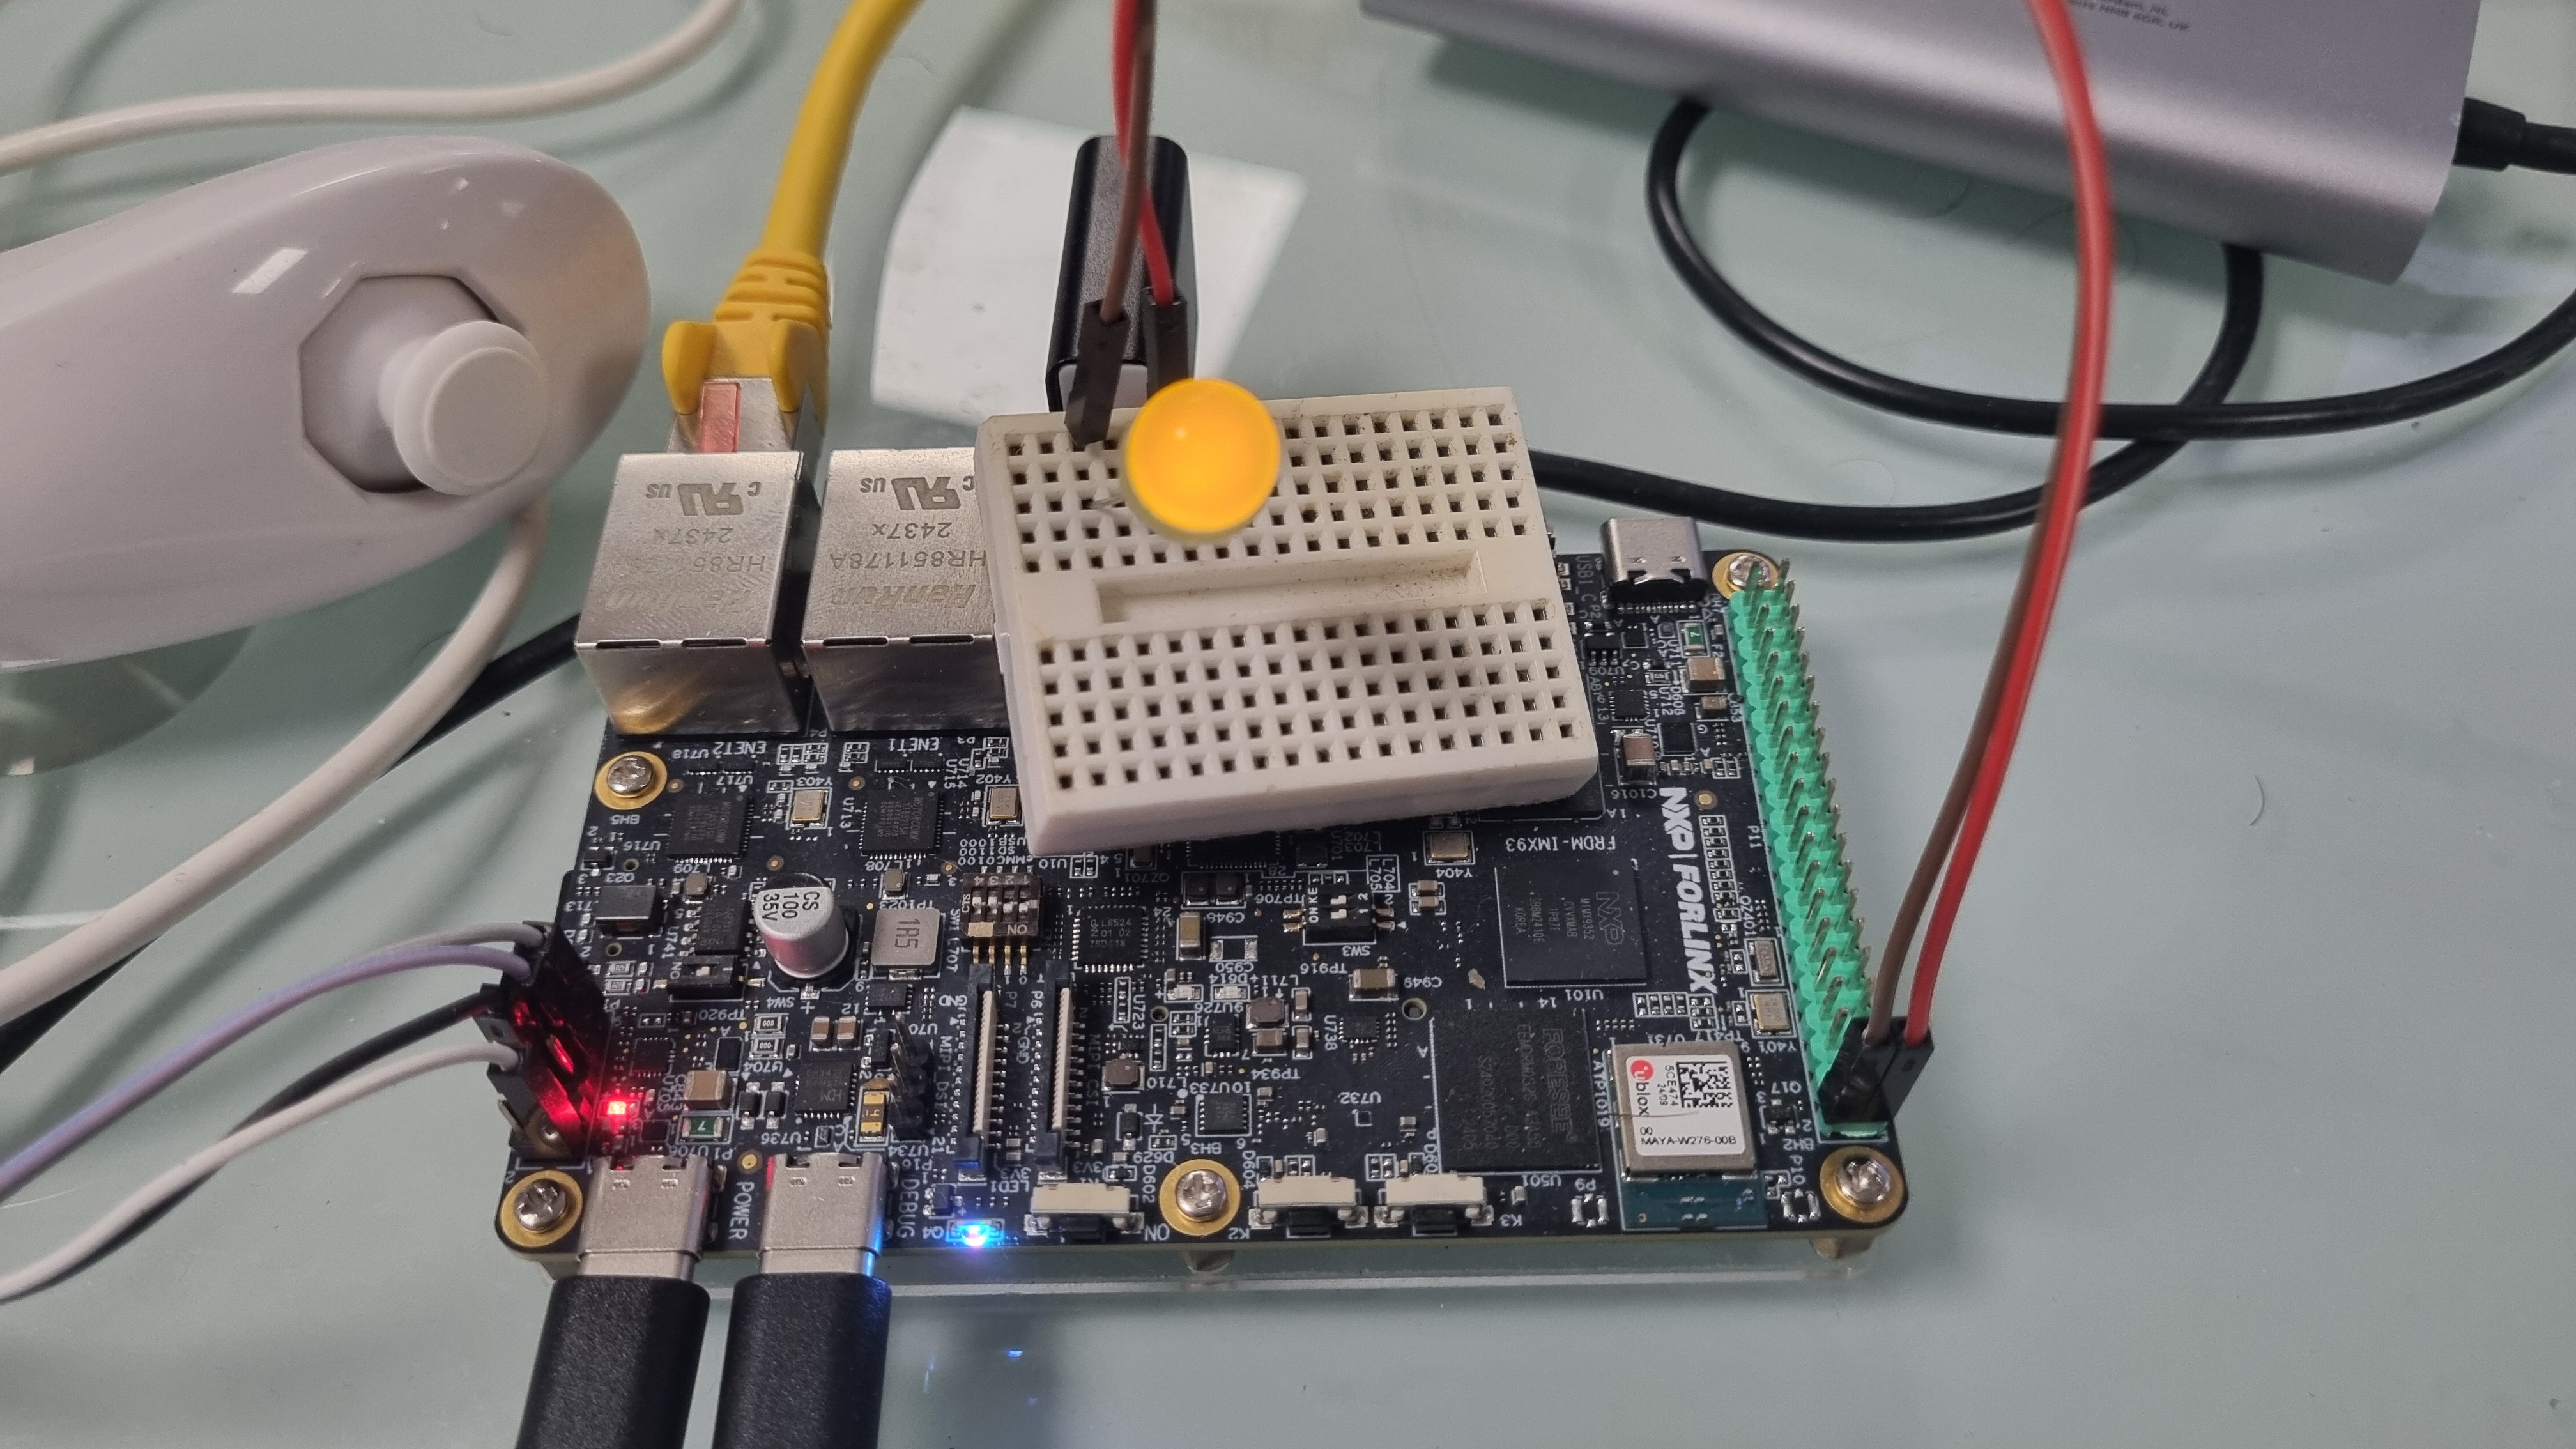
\includegraphics[height=0.3\textheight]{slides/sysdev-hw-devices/imx93-frdm/led-on.jpg}
  \end{center}
  \end{columns}
\end{frame}

\begin{frame}[fragile]{Example: connect I2C temperature, humidity and pressure sensor}
  \begin{columns}
    \column{0.5\textwidth}
    \begin{block}{imx93-11x11-frdm-custom.dts}
      {\tiny
\begin{minted}{perl}

&lpi2c4 {
  #address-cells = <1>;
  #size-cells = <0>;
  clock-frequency = <400000>;
  pinctrl-names = "default", "sleep";
  pinctrl-0 = <&pinctrl_lpi2c4>;
  pinctrl-1 = <&pinctrl_lpi2c4>;
  status = "okay";

    pressure@76 {
            compatible = "bosch,bme280";
            reg = <0x76>;
    };
};

\end{minted}
}
  \end{block}

\begin{block}{shell}
{\tiny
\begin{verbatim}
# cat /sys/bus/iio/devices/iio\:device2/in_humidityrelative_input
49147
# cat /sys/bus/iio/devices/iio\:device2/in_pressure_input
101.567167968
# cat /sys/bus/iio/devices/iio\:device2/in_temp_input
24380
\end{verbatim}
}
\end{block}
  \column{0.5\textwidth}
  \begin{center}
    \includegraphics[width=0.4\textwidth]{slides/sysdev-hw-devices/bme.jpg}
  \end{center}
\end{columns}
\end{frame}

\begin{frame}{Further details about the Device Tree}
\small
Check out our {\em Device Tree 101 webinar}, by Thomas Petazzoni (2021)
\begin{itemize}
    \item Slides: \url{https://bootlin.com/blog/device-tree-101-webinar-slides-and-videos/}\\
    \item Video: \url{https://youtu.be/a9CZ1Uk3OYQ}
\end{itemize}
\vspace{0.5cm}
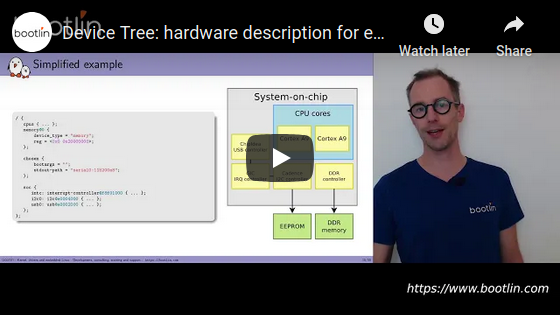
\includegraphics[height=0.5\textheight]{common/device-tree-video.jpg}
\end{frame}

\subsection{Discoverable hardware: USB and PCI}

\begin{frame}{Discoverable hardware}
  \begin{itemize}
  \item Some busses have built-in hardware discoverability mechanisms
  \item Most common busses: USB and PCI
  \item Hardware devices can be enumerated, and their characteristics
    retrieved with just a driver or the bus controller
  \item Useful Linux commands
    \begin{itemize}
    \item \code{lsusb}, lists all USB devices detected
    \item \code{lspci}, lists all PCI devices detected
    \item A detected device does not mean it has a kernel driver
      associated to it!
    \end{itemize}
  \item Association with kernel drivers done based on product
    ID/vendor ID, or some other characteristics of the device: device
    class, device sub-class, etc.
  \end{itemize}
\end{frame}

\setuplabframe
{Accessing hardware devices}
{
  Time to start the practical lab!
  \begin{itemize}
  \item Exploring the contents of \code{/dev} and \code{/sys} and the
    devices available on the embedded hardware platform.
  \item Using GPIOs and LEDs.
  \item Modifying the Device Tree to control pin multiplexing and
        declare an I2C-connected joystick.
  \item Adding support for a USB audio card using Linux kernel modules
  \item Adding support for the I2C-connected joystick through
        an out-of-tree module.
  \end{itemize}
}
